\documentclass{article}
\usepackage{amsmath}
\usepackage{graphicx}
\usepackage{listings}  % Include this package to define lstlisting environment
\UseRawInputEncoding
\usepackage{color}
\lstset{ 
  basicstyle=\ttfamily,
  columns=fullflexible,
  frame=single,
  breaklines=true,
  postbreak=\mbox{\textcolor{red}{$\hookrightarrow$}\space},
}

\title{Real Data Analysis: Comparing Parametric and Nonparametric Methods(Statistical Analysis of Alcohol Levels in
Wine Dataset)}
\author{Chandrika Kunchakuri}
\date{\today}

\begin{document}

\maketitle

\section{Introduction}
This report details the analysis strategy for comparing alcohol levels between different classes of wine using both parametric and nonparametric statistical methods. The dataset includes alcohol measurements obtained through teaching techniques well as technology enhanced learning methodologies.

\section{Data Description}
\subsection{Individuals in the Sample}
The Wine Dataset contains information about various chemical properties of wines, including alcohol levels, malic acid content, ash content, magnesium etc.
The sample consists of 173 samples divided into three groups:
\begin{itemize}
    \item Class 1: 59 instances 
    \item Class 2: 71 instances
    \item Class 3: 48 instances
\end{itemize}

\subsection{Actual Data Values(or data set link)}
\textbf{UC Irvine Test Data url:} https://archive.ics.uci.edu/ml/machine-learning-databases/wine/wine.data
\newpage
\section{Research Question}
\begin{flushleft}\textbf{Research Question:} Is there a significant difference in alcohol levels between the different classes of wine taught by traditional methods and those taught by technology-assisted methods?

\textbf{Null Hypothesis \( H_0 \):}There is no difference in the mean alcohol levels between the different classes of wine.

\textbf{Alternative Hypothesis \( H_A \):} There is a difference in the mean alcohol levels between the different classes of wine.

\end{flushleft}
\section{Suggested Approaches}
\subsection{Nonparametric Approach}
In our nonparametric analysis, we will use the Mann-Whitney U test. This test is based on assumptions;
\\1) Random Sampling: Samples are taken randomly from the population.
\\2) Independence: Observations within each group are independent of each other.
\\3) Continuous or Ordinal Data: The data needs to be measurable on at an ordinal scale.
\\4) It also doesn't assume a normal distribution of alcohol levels among different classes of wine.
%, which is appropriate as it does not assume a normal distribution of the scores.

\subsection{Parametric Approach}
To analyze without parameters we'll employ the One way ANOVA test to compare the alcohol levels, across wine categories. 
\\Here are the key assumptions:
\\1) Normality: The data within each group follows a normal distribution.
\\2) Homogeneity of Variance: The variance of the data is approximately equal across all groups.
\\3) Independence: Observations within each group are not influenced by one another.
%, assuming equal variances, to compare the means of the two groups.

\section{Statistical Analysis, Plots and Observations}
The codes for Statistical Analysis (Mann-Whitney U Test and One-way ANOVA) and Plots (Power plot and Normal plot) are placed in appendix.

% Here you would include commands to generate and include plots, such as histograms or box plots of the data.
% You would also include LaTeX code for plotting the power functions, assuming hypothetical values or simulations.
\subsection{Analysis} 
\begin{figure}[ht]
    \centering
    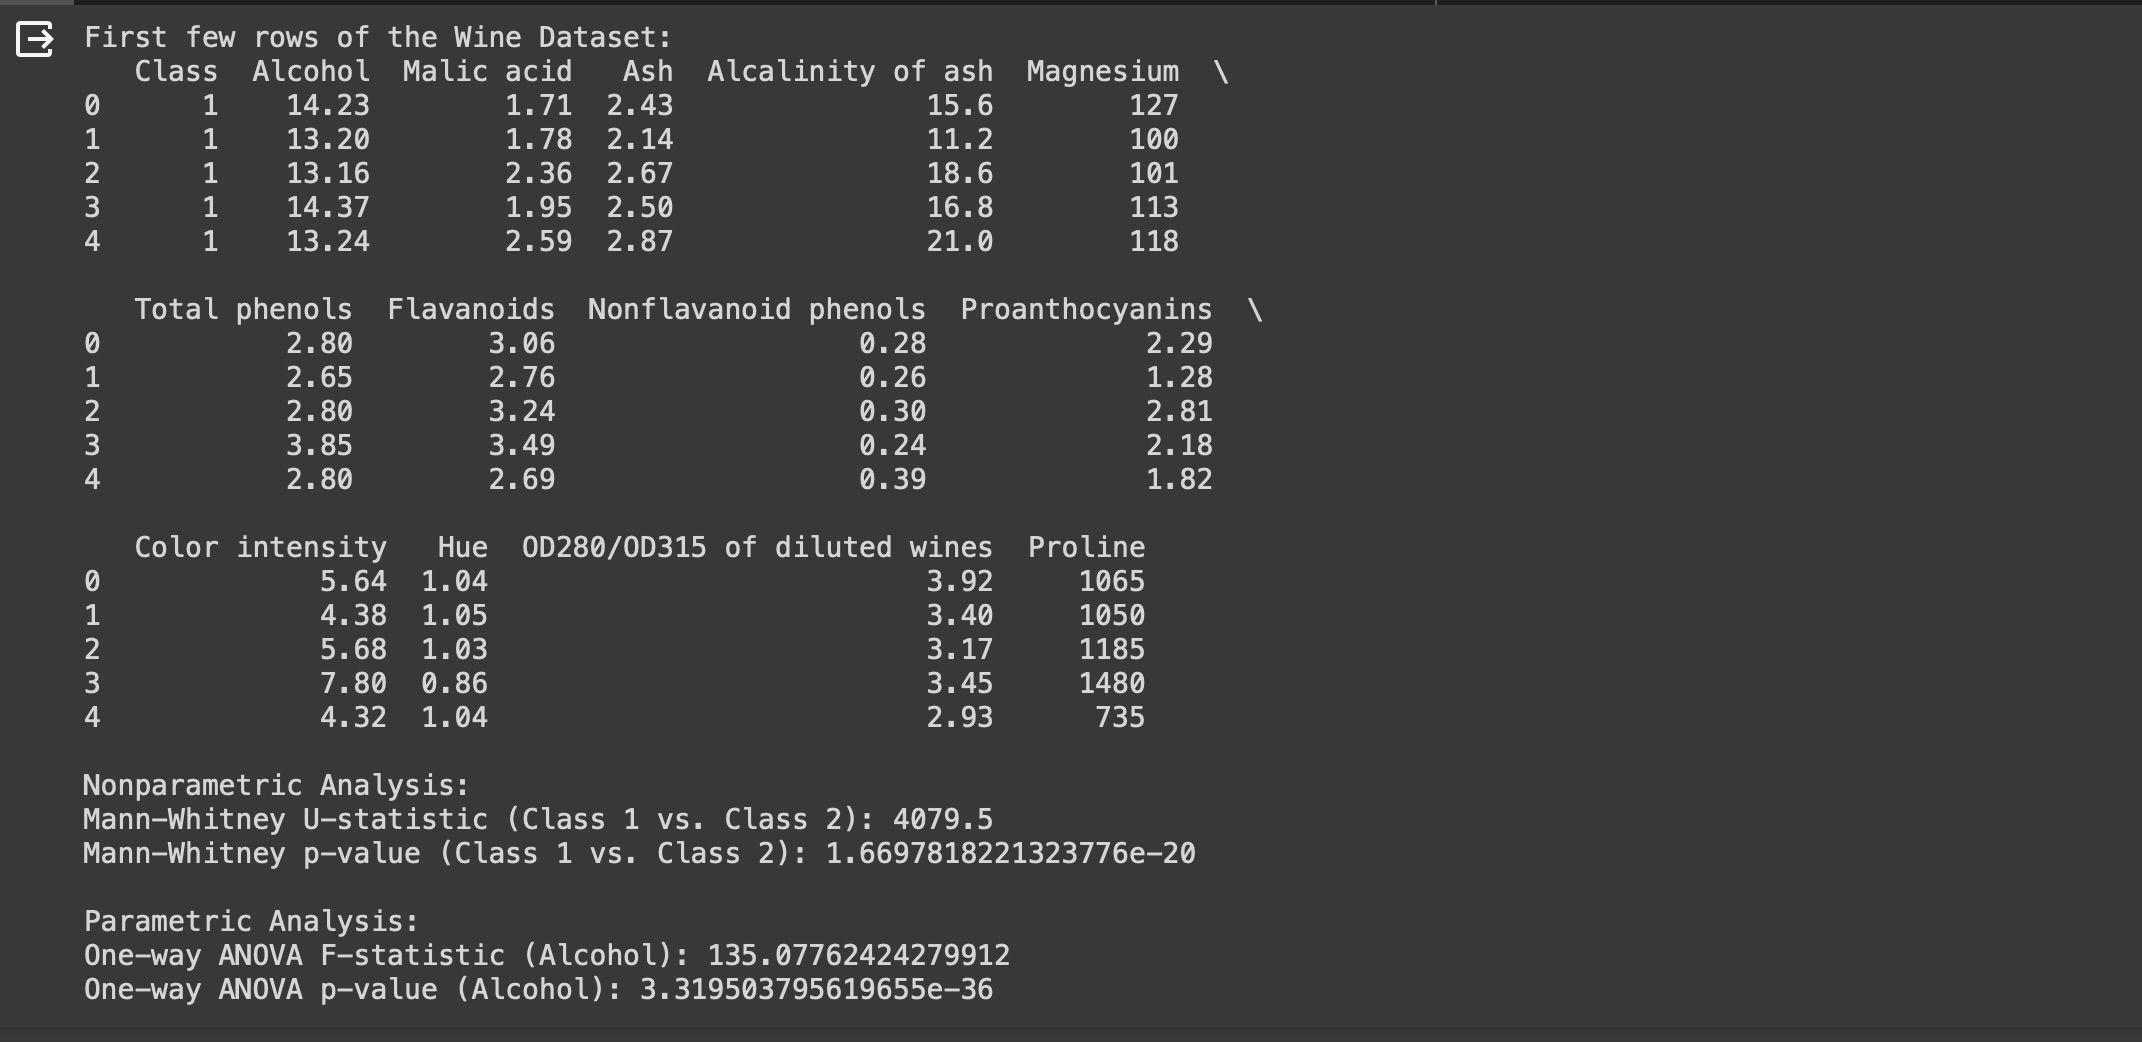
\includegraphics[width=0.7\linewidth]{StatAnalysis.jpeg}
    \caption{Parametric and NonParametric Analysis of Alcohol levels in Wine Dataset}
    \label{fig:AnalysisResult}
\end{figure}
1)First few rows of the Wine Dataset:
Here are the initial rows of the Wine Dataset showcasing characteristics of wines like alcohol content, malic acid content and ash content. Each row corresponds to a wine sample, and each column represents a different chemical property.
\subsubsection {Non Parametric Analysis}
Mann-Whitney U statistic (Class 1 vs. Class 2): The Mann-Whitney U statistic gauges the magnitude difference between two groups by comparing alcohol levels in Class 1 and Class 2 wines. The U statistic value stands at 4079.5.
\\Mann-Whitney p value (Class 1 vs. Class 2): The p-value associated with the Mann-Whitney U test measures the strength of evidence against the null hypothesis, which states that there is no difference in alcohol levels between Class 1 and Class 2 wines. 
\\The p value is extremely small $1.67 \times 10^{-20}$ indicating evidence against the null hypothesis. Therefore, we reject the null hypothesis and conclude that there is a significant difference in alcohol levels between Class 1 and Class 2 wines.

\subsubsection {Parametric Analysis}
One-way ANOVA F-statistic (Alcohol): The F-statistic from the one-way ANOVA test measures the ratio of the variance between groups to the variance within groups in terms of alcohol levels across Class 1, Class 2 and Class 3 wines. The F statistic value is recorded at 135.08.
\\One-way ANOVA p-value (Alcohol): The p-value associated with the one-way ANOVA test measures the strength of evidence against the null hypothesis, which states that there is no difference in alcohol levels among the three classes of wines. 
\\The p value is remarkably small at around $3.32 \times 10^{-36}$ suggesting evidence against this hypothesis. Consequently we can reject the hypothesis and conclude that there is a significant difference in alcohol levels among the three classes of wines.

\newpage
\subsection {Inferences from Power Analysis}
Based on the power analysis: 
\begin{itemize}
\item One way ANOVA demonstrates power across varying sample sizes. Its power is slightly higher for smaller sample sizes and stabilizes with larger samples. This indicates that One way ANOVA is robust and consistent in detecting differences in effect size across sample sizes.
\item Similarly, power of the Mann-Whitney U Test remains relatively stable across different sample sizes. This suggests that the test is reliable and consistent in detecting differences in effect size of sample sizes.
\item Notably, when dealing with smaller samples and a moderate effect size (0.5), the One way ANOVA test often shows more power compared to Mann-Whitney U Test.
\item Ordinal: The alcohol values in the dataset are continuous numerical variables representing the alcohol content of wine samples. They are not ordinal since they represent a quantitative measurement rather than a categorical ranking.
\end{itemize}
\vspace{0.5in}
\begin{figure}[ht]
    \centering
    \includegraphics[width=0.6\linewidth]{PowerAnalysis.png}
    \caption{Power Analysis of Alcohol Levels in Wine Dataset}
    \label{fig:PowerAnalysis}
\end{figure}

\newpage
\subsection {Observations from Normal Plot}
 The normal plot of alcohol levels in the wine dataset provides insights into the distributional characteristics of the data. Here's an overview:
\begin{itemize}
\item Shape of the Distribution: The histogram, combined with the kernel density estimation (KDE) curve illustrates how alcohol levels are distributed in the dataset. The shape of the distribution resembles a bell-shaped curve indicating to normal distribution.
\item Symmetry: This balanced/symmetric bell-shaped curve suggests that there's an equal chance of finding alcohol levels above and below the mean value indicating symmetry around the mean. 
\item Center of the Distribution: The peak of the curve represents the mean alcohol level in the dataset reflecting the most common or typical levels found in the wines. 
\item Spread of the Distribution: The spread or variability of alcohol levels is captured by the width of the curve. A wider curve indicates higher variability while a narrower one suggests lower variability. In this plot, the curve seems moderate pointing to a moderate level of variability among wine alcohol levels.
\item Outliers, if present, would appear as data points that deviate significantly from the main body of the distribution. In this plot, there are no obvious outliers visible, indicating that the majority of alcohol level values fall within a reasonable range.
\end{itemize}
\begin{figure}[ht]
    \centering
    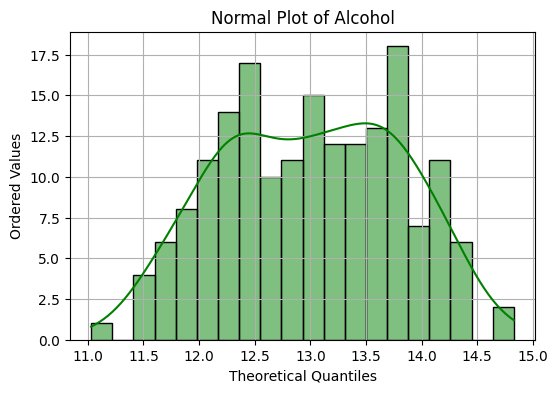
\includegraphics[width=0.6\linewidth]{NormalPlot.png}
    \caption{Normal Plot of Alcohol Levels in Wine Dataset}
    \label{fig:NormalPlot}
\end{figure}
Overall, the normal plot of alcohol levels provides visual confirmation that the data follows an approximately normal distribution, which is an important assumption for many parametric statistical analyses.
\newpage
\section{Conclusions}
Preferred Testing Method:

1)Significant Differences in Alcohol Levels: Both parametric and nonparametric analyses consistently indicate significant differences in alcohol levels between different classes of wine. The small p value obtained from both the Mann-Whitney U test and the one-way ANOVA test reject the null hypothesis, providing strong evidence that there are indeed differences in mean alcohol levels among the wine classes.

2)If the data meet the assumptions of the one-way ANOVA (normality, homogeneity of variances) and the research question involves comparing means across multiple groups, then the one-way ANOVA may be preferred.

3)If the data do not meet the assumptions of parametric tests or if the research question involves ordinal or non-normally distributed data, the Mann-Whitney U test can be a suitable alternative.

4)In this context of the wine dataset analysis, from the power analysis, for smaller sample sizes, the One-way ANOVA(red line) tends to have slightly higher power compared to Mann-Whitney U test(red line), especially when the effect size is moderate (0.5).

So, One-way ANOVA is preferrable over the Mann-Whitney U test. 
\\2)The Mann-Whitney U test: 
\\Advantages:

a)Nonparametric tests that does not assume normality or equal variances.

b)Suitable for ordinal or continuous data that may not follow a normal 

distribution.

c)Robust to outliers and skewed data.
\\Considerations:

a)Less powerful than parametric tests when data truly follows a normal 

distribution.

b)May have reduced sensitivity with smaller sample sizes.

c)Does not provide information about specific group differences beyond 

ranking.
\\3)The one-way ANOVA test: 
\\Advantages:

a)Parametric test that assumes normality and equal variances, which can be 

more powerful when these assumptions are met.

b)Provides information about specific group differences and interactions.

c)Allows for analysis of multiple groups simultaneously.
\\Considerations:

a)Sensitive to violations of assumptions such as normality and homogeneity

of variances.

b)Less robust to outliers and skewed distributions.

c)Requires larger sample sizes to maintain statistical power, especially

when assumptions are violated.

\newpage
\appendix
\section{Appendix: Statistical Analysis Code}
\subsection{Python Code to load the Test Data}
\begin{lstlisting}[language=Python]
# Python Code to load the Test Data
import pandas as pd
from scipy.stats import mannwhitneyu, f_oneway
# Load the Wine Dataset
url = "https://archive.ics.uci.edu/ml/machine-learning-databases/wine/wine.data"
column_names = ["Class", "Alcohol", "Malic acid", "Ash", "Alcalinity of ash", 
                "Magnesium", "Total phenols", "Flavanoids", "Nonflavanoid phenols", 
                "Proanthocyanins", "Color intensity", "Hue", "OD280/OD315 of diluted wines", 
                "Proline"]
wine_data = pd.read_csv(url, header=None, names=column_names)

# Display the first few rows of the dataset
print("First few rows of the Wine Dataset:")
print(wine_data.head())
\end{lstlisting}
\subsection{Python Code for One-way ANOVA}
\begin{lstlisting}[language=Python]
# Nonparametric Analysis(Mann-Whitney U test)
class_1_alcohol = wine_data[wine_data['Class'] == 1]['Alcohol']
class_2_alcohol = wine_data[wine_data['Class'] == 2]['Alcohol']
u_statistic, p_value = mannwhitneyu(class_1_alcohol, class_2_alcohol)
print("\nNonparametric Analysis:")
print("Mann-Whitney U-statistic (Class 1 vs. Class 2):", u_statistic)
print("Mann-Whitney p-value (Class 1 vs. Class 2):", p_value)
\end{lstlisting}
\subsection{Python Code for Mann-Whitney U Test}
\begin{lstlisting}[language=Python]
# Parametric Analysis(One-way ANOVA)
class_1_alcohol = wine_data[wine_data['Class'] == 1]['Alcohol']
class_2_alcohol = wine_data[wine_data['Class'] == 2]['Alcohol']
class_3_alcohol = wine_data[wine_data['Class'] == 3]['Alcohol']
f_statistic, p_value = f_oneway(class_1_alcohol, class_2_alcohol, class_3_alcohol)
print("\nParametric Analysis:")
print("One-way ANOVA F-statistic (Alcohol):", f_statistic)
print("One-way ANOVA p-value (Alcohol):", p_value)
\end{lstlisting}
\subsection{Python Code for Power Analysis}
\begin{lstlisting}[language=Python]
import numpy as np
import matplotlib.pyplot as plt
from scipy.stats import mannwhitneyu
from statsmodels.stats.power import TTestIndPower
Class_a = class_1_alcohol
Class_b = class_2_alcohol
alpha = 0.05
sample_sizes = np.arange(5, 26)
power_mw = [mannwhitneyu(np.random.choice(Class_a, size=n), np.random.choice(Class_b, size=n))[1] for n in sample_sizes]
effect_size = np.abs(Class_a.mean() - Class_b.mean()) / np.sqrt((Class_a.var() + Class_b.var()) / 2)
ttest_power = TTestIndPower()
power_t = [ttest_power.solve_power(effect_size=effect_size, nobs1=n, alpha=alpha, alternative='two-sided') for n in sample_sizes]
plt.plot(sample_sizes, power_mw, color='blue', label='MW_Test',linewidth=2)
plt.plot(sample_sizes, power_t, color='red', label='t-Test',linewidth=2)
plt.xlabel('Sample_Size')
plt.ylabel('Power')
plt.title('Power_Curve_Comparison')
plt.axhline(alpha, color='black', linestyle='--', label='Significance␣Level')
plt.legend()
plt.show()
\end{lstlisting}
\newpage
\subsection{Python Code for Normal Plot of Alcohol}
\begin{lstlisting}[language=Python]
import numpy as np
import pandas as pd
import seaborn as sns
import matplotlib.pyplot as plt
import scipy.stats as stats

# Load the Wine Dataset
url = "https://archive.ics.uci.edu/ml/machine-learning-databases/wine/wine.data"
column_names = ["Class", "Alcohol", "Malic acid", "Ash", "Alcalinity of ash", 
                "Magnesium", "Total phenols", "Flavanoids", "Nonflavanoid phenols", 
                "Proanthocyanins", "Color intensity", "Hue", "OD280/OD315 of diluted wines", 
                "Proline"]
df = pd.read_csv(url, header=None, names=column_names)

# Extract alcohol values for plotting
alcohol_values = df['Alcohol']
plt.figure(figsize=(6, 4))
sns.histplot(df['Alcohol'], kde=True, color='green', bins=20)
plt.title('Normal Plot of Alcohol')
plt.xlabel('Theoretical Quantiles')
plt.ylabel('Ordered Values')
plt.grid(True)
plt.show()
\end{lstlisting}
\end{document}
